% вторая часть

\section{Разработка приложения}

\subsection{Обзор инструментов разработки}

Для разработки приложения на основании требований, описанных в \ref{trebovaniya}, были выбраны следующие инструменты:

\subsubsection{Python}

Язык программирования Python - высокоуровневый, интерпретируемый, объектно-ориентированный язык программирования, который широко используется для разработки веб-приложений, научных вычислений, анализа данных, искусственного интеллекта, автоматизации задач и многих других областей. В совокупности с большим набором пользовательских библиотек, python предоставляет мощные инструменты для обработки, анализа и визуализации данных. 

В качестве альтернативы Python рассматривался язык R. R предоставляет более широкий спектр функций по обработке и анализу данных, но набор инструментов для визуализации, а также создания интерфейса приложений ограничен. Именно этот фактор стал решающим в пользу Python.

\subsubsection{Pandas + NumPy}

NumPy (Numerical Python) --- это библиотека для работы с массивами и матрицами, а также для выполнения математических операций над ними. Преимущество NumPy заключается в дешевизне операций и скорости работы, что делает ее неотъемлемым инструментом для анализа данных, машинного обучения, статистики и других областей, где требуется работа с табличными данными.

Pandas --- это библиотека для анализа данных, построенная на основе NumPy. Она предоставляет высокоуровневые структуры данных и инструменты для работы с табличными и временными рядами данных.

Совместное использование Pandas и NumPy позволяет эффективно решать широкий спектр задач в области научных исследований, финансового анализа, обработки больших данных и машинного обучения. NumPy обеспечивает высокую производительность при выполнении числовых вычислений, тогда как Pandas предоставляет удобные инструменты для обработки и анализа данных. Вместе эти библиотеки образуют мощный инструментарий для решения задач, связанных с анализом и обработкой данных в Python.



%Библиотека Pandas -  программная библиотека на языке Python для обработки и анализа данных. Работа Pandas с данными строится поверх библиотеки NumPy, являющейся инструментом более низкого уровня. Предоставляет специальные структуры данных и операции для манипулирования табличными данными. Преимущество NumPy заключается в дешевизне операций и скорости работы, что делает ее неотъемлемым инструментом для анализа данных, машинного обучения, статистики и других областей, где требуется работа с табличными данными.

%\subsubsection{NumPy}

%Библиотека NumPy предоставляет эффективные контейнеры для
%работы с массивами и матрицами данных. В совокупности с Pandas она широко используется для выполнения математических операций и вычислений в Python.

\subsubsection{SciPy}

SciPy --- библиотека, основанная на расширении NumPy, которая применяется для более сложных научных и инженерных вычислений. SciPy в основном написана на Python и частично на языках C, C++ и Fortran, в связи с чем отличается высокой производительностью и скоростью работы. В рамках разработки приложения использовался модуль scipy.stats, который предоставляет обширный функционал для проведения статистических вычислений.

\subsubsection{Matplotlib+Seaborn}

Библиотеки Matplotlib и Seaborn. Эти библиотеки предоставляют
возможности для визуализации данных в Python. Matplotlib является основной
библиотекой для создания различных типов графиков, в то время как Seaborn
предоставляет более высокоуровневый интерфейс для создания
статистических графиков.

\subsubsection{PyQt}

PyQt --- набор расширений кроссплатформенного графического фреймворка Qt, выполненный в виде библиотеки Python. Qt --- фреймворк для разработки кроссплатформенного программного обеспечения c графическим интерфейсом, написанный на языке программирования C++.

Базовыми элементами графического интерфейса PyQt являются виджеты(Widgets) --- основные строительные блоки для создания графических интерфейсов пользователя. PyQt предоставляет широкий ассортимент виджетов, которые можно использовать для построения сложных и функциональных приложений. Виджеты в PyQt охватывают разнообразные элементы, такие как кнопки, текстовые поля, метки, списки и многое другое. В этом тексте мы рассмотрим основные виды виджетов и их использование в PyQt.

PyQt использует систему сигналов и слотов для реализации взаимодействия с пользователем. Сигналы используются для уведомления об изменениях состояния, а слоты — для обработки этих изменений.

\subsection{Импорт данных}

На первом этапе разработки необходимо реализовать импорт входных данных из формата .ods. Пример модельных данных представлен на рисунках \ref{fig:ris4}-\ref{fig:ris5} 

\begin{figure}[H]
	\centering
	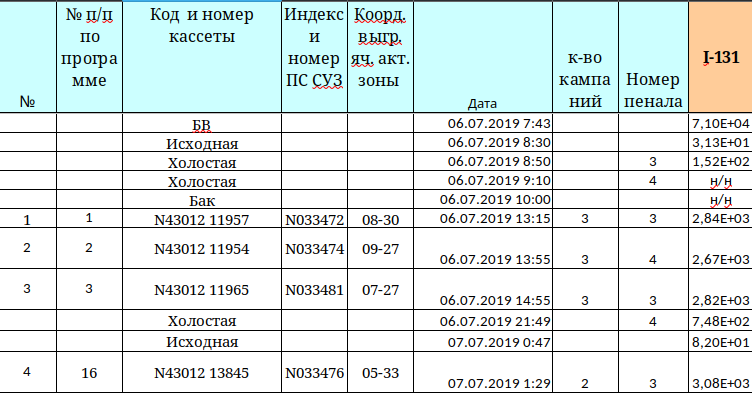
\includegraphics[width=1\linewidth]{pics/ris4} % изображения хранятся в подкаталоге pics
	\caption{Пример входных данных}
	\label{fig:ris4} % эта метка позволяет ссылаться на рисунок в тексте
\end{figure}

\begin{figure}[H]
	\centering
	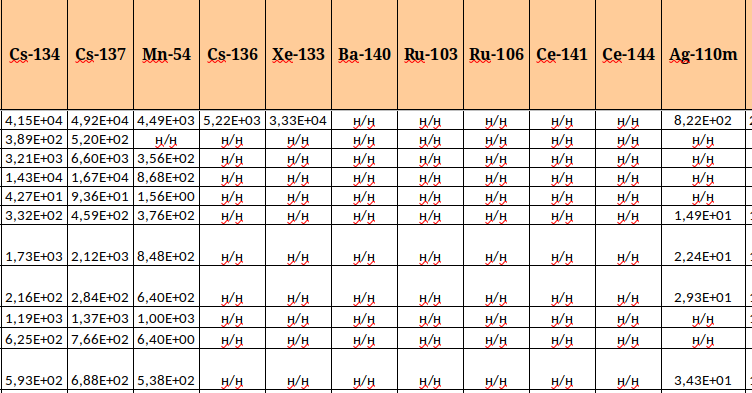
\includegraphics[width=1\linewidth]{pics/ris5} % изображения хранятся в подкаталоге pics
	\caption{Пример входных данных}
	\label{fig:ris5} % эта метка позволяет ссылаться на рисунок в тексте
\end{figure}

Как видно из примера, входные данные содержат строки и столбцы, которые используются в других расчётах. Следовательно, для использования в приложении эти данные необходимо очистить. 

Чтение файла из табличных файлов(таких как .xls, .xlsx, .ods) реализовано в методе read\_excel() библиотеки pandas. Данная функция возвращает объект DataFrame, который передаётся в метод очистки под определённый шаблон входных данных. Фрагмент реализация метода, отвечающего за очистку DataFrame представлена на листинге~\ref{lst:1}. 

\begin{flushleft}
\needspace{3\baselineskip}
\captionof{Program}{Метод очистки данных} \label{lst:1}
\begin{MyCodes}
def _clear_data(self, df):
	# На текущий момент данные очищаются под конкретный шаблон пробных данных.
	# Делаем срез DataFrame, используем первые 14 столбцов
	df = df.iloc[:,0:14] 
	# Переименовываем столбцы для удобного анализа
	df.rename(columns = {
		"№":"Id1",
		"№ п/п по программе":"Id2",
		"Код  и номер кассеты":"Name",
		"Индекс и номер ПС СУЗ":"Index",
		"Коорд. выгр. яч. акт. зоны ":"Coordinates",
		"Дата":"DateTime",
		"к-во кампаний":"Age",
		"Номер пенала":"IdPenal"}, inplace = True)
	
	for i in range(0, len(df.columns.to_list())):
		column = df.columns.to_list()[i]
		df.replace({column:"-"}, np.NaN, inplace=True) # Заменяем спец. символы
		df.replace({column:"н/н"}, np.NaN, inplace=True)
	
	# Заполняем пропуски и приводим типы
	df["Age"]=df["Age"].fillna(0.0).astype(int)
	df["IdPenal"]=df["IdPenal"].fillna(0.0).astype(int)
	df["Id2"]=df["Id2"].fillna(0.0).astype(int)
	
	...
	
	return penals, penals_id, cassetes

\end{MyCodes}
\end{flushleft}

\subsection{Анализ данных}

\subsection{Пользовательский интерфейс}

Данный раздел содержит описание инструментов и трудностей, с которыми я столкнулся во время разработки приложения, а также примеры реализаций графических элементов, используемых в моём приложении.

\subsubsection{Основные окна приложения}

На основании анализа пользовательского сценария использования, представленного в \ref{Scenarii}, был сделан вывод, что проектируемое приложение будет состоять 4 окон(2 основных и 2 диалоговых):

\begin{itemize}
	\item Диалоговое окно импорта файла
	\item Окно анализа пеналов
	\item Окно анализа выборок
	\item Диалоговое окно с результатами статистических тестов 
\end{itemize}



\subsubsection{Окно импорта файла}

При открытии файла используется класс QFileDialog, который предоставляет окно выбора файла. Удобство этого класса заключается в том, что имеется возможность установить фильтры на расширения файлов, чтобы не вызывать исключений при попытке открыть файл с расширением, которое не поддерживается. Пример окна для выбора фала представлен на рисунке~\ref{fig:ris7}.

\begin{figure}[H]
	\centering
	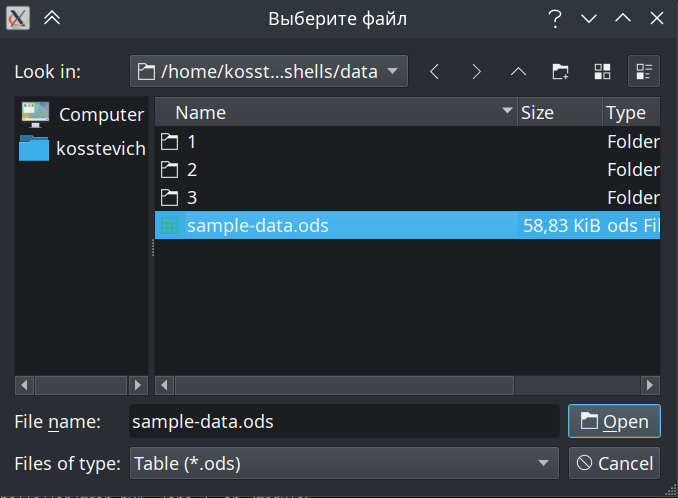
\includegraphics[width=1\linewidth]{pics/ris7} % изображения хранятся в подкаталоге pics
	\caption{Окно выбора файла}
	\label{fig:ris7} % эта метка позволяет ссылаться на рисунок в тексте
\end{figure}

\subsubsection{Интеграция Matplotlib в качестве QWidget}

Во время разработки приложения я столкнулся с трудностью интеграции графиков Matplotlib в QWidjet. Проблема заключалась в том, что базовый класс Matplotlib создаёт для графиков независимые окна. Данная реализация мне не подходит, т.к. разрабатываемое приложение должно иметь целостный формат.

Изучив документацию библиотеки, я нашёл класс FigureCanvasQTAgg, предоставляющий backend-реализацию холста Canvas для PyQt. На основе него был разработан собственный пользовательский виджет для использования в моём приложении. Реализация пользовательского виджета представлена в листинге~\ref{lst:canvas}

\begin{flushleft}
\needspace{3\baselineskip}
\captionof{Program}{Пользовательский класс, интегрирующий Сanvas в QWidget} \label{lst:canvas}
\begin{MyCodes}
class PlotData(FigureCanvasQTAgg): 
	# Виджет для отрисовки графиков, использующий matplotlib
	def __init__(self, parent=None):
		sns.set(style="whitegrid", context="paper")
		self.fig = plt.figure(figsize=(15, 10))
		self.axes = self.fig.add_subplot(111)
		super(PlotData, self).__init__(self.fig)
	
	def draw_plot(self, df, axe_x="Id1",
			axe_y="I-131", type = "barplot", name=None):
		self.axes.cla()
		# Метод позволяет рисовать разные виды графиков seaborn
		# Выбор типа графика происходит по аргументу type
		getattr(sns,type)(data=df, x=axe_x, y=axe_y, ax=self.axes)
		plt.title(label= name, fontsize=16)
\end{MyCodes}
\end{flushleft}

Кроме реализации холста я использовал класс NavigationToolbar2QT, который предоставляет возможности навигации, редактирования легенды, а также экспорт графика в формате изображения. На рисунке~\ref{fig:ris8} красной рамкой выделены реализованные мною классы.

\begin{figure}[H]
	\centering
	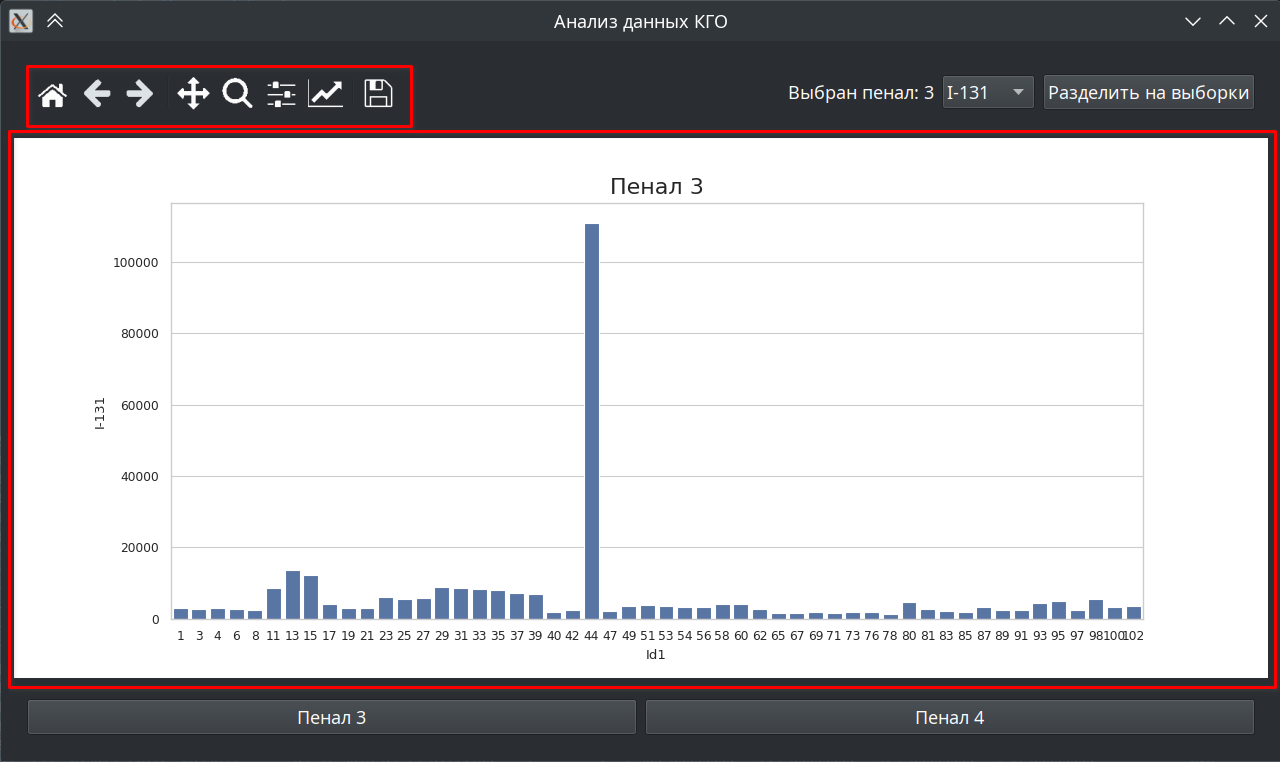
\includegraphics[width=0.96\linewidth]{pics/ris8} % изображения хранятся в подкаталоге pics
	\caption{Главное окно приложения}
	\label{fig:ris8} % эта метка позволяет ссылаться на рисунок в тексте
\end{figure}

\subsubsection{Главное окно приложения}


%Интеграция графиков Matplotlib в QtWidget